\documentclass[12pt]{article}
\usepackage{listings}
\usepackage[colorlinks=true,pagebackref,linkcolor=blue]{hyperref}
\usepackage{graphicx}
\usepackage{tikz}
\textwidth=7in
\textheight=9.5in
\topmargin=-1in
\headheight=0in
\headsep=.5in
\hoffset  -.85in

\lstset{
basicstyle=\footnotesize\ttfamily,
language=bash,
upquote=true,
breakatwhitespace=true,
columns=fullflexible,
keepspaces,
%numbers=none,
tabsize=3,
frame=blrt,
framextopmargin=5pt,
showstringspaces=false,
extendedchars=true
}

\pagestyle{empty}

\renewcommand{\thefootnote}{\fnsymbol{footnote}}

\begin{document}



\begin{center}
{\bf AMS 550.400 \quad Revised HW SET 1\quad  Due Date:  Oct 31}\\
\vskip.2in
{\footnotesize Last Compiled on \today}
\\Zhendan Zhu
\end{center}

\setlength{\unitlength}{1in}

\begin{picture}(6,.1) 
\put(0,0) {\line(1,0){6.25}}         
\end{picture}

 

\renewcommand{\arraystretch}{2}


\vskip.25in
\noindent\textbf{Problem 1 (10 pts):}  
\noindent\textbf{}
\\
In this problem, I used the following code:  
  \\  cd \textasciitilde/550400
  \\  mkdir \textasciitilde/550400/honda
  \\  cd \textasciitilde/550400/honda
  \\  git init
  \\  vi main.txt
  \\  git add .
  \\  git commit -m "A is done"
  \\  vi main.txt
  \\  git add .
  \\  git commit -m"B is done"
  \\  git checkout -b alt
  \\  vi main.txt
  \\  git add .
  \\  git commit -m"X is done"
  \\  git checkout master
  \\  vi main.txt
  \\  git add .
  \\  git commit -m "C is done"
  \\  git merge alt
  \\  vi main.txt
  \\  vi main.txt
  \\  git add .
  \\  git commit -m "D is done"
  \\  git log --graph --oneline
  \\  git checkout alt
  \\  git log --graph --oneline
  \\  git push https://github.com/zhendanzhu/honda.git master
  \\  git push https://github.com/zhendanzhu/honda.git alt
\\The graphs are as following:

\begin{figure}[h]
    \begin{center}
        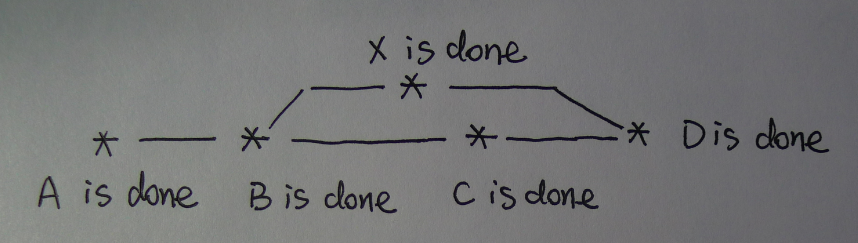
\includegraphics[scale=0.3]{grapha.png}
    \end{center}
    \caption{The history graph for master branch}
    \label{fig:branch}
\end{figure}

\begin{figure}[h]
    \begin{center}
        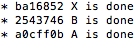
\includegraphics[scale=0.3]{graphb.png}
    \end{center}
    \caption{The history graph for alt branch}
    \label{fig:branch}
\end{figure}


\newpage
\vskip.25in
\noindent\textbf{Problem 2 (10 pts):}
\noindent\textbf
\\mkdir newpoem
\\cd  \textasciitilde/newpoem
\\git config --global user.name "zhendanzhu"
\\git config --global user.email zhendanzhu@hotmail.com
\\git remote add stanza1 git://github.com/nhlee/550400.stanza1.git 
\\git remote add stanza2 git://github.com/nhlee/550400.stanza2.git 
\\git remote add stanza3 git://github.com/nhlee/550400.stanza3.git 
\\git init
\\git checkout master
\\git pull stanza1 master
\\vi  main.txt
\\git add .
\\git commit -m " add a title "
\\git checkout -b alt1
\\git pull stanza2
\\git checkout master
\\git merge alt1
\\vi main.txt
\\git add .
\\git commit -m "resolve conflict1"
\\git checkout -b alt2
\\git pull stanza3
\\git checkout master
\\vi main.txt
\\git add .
\\git commit -m "resolve conflict2"
\\git remote add origin https://github.com/zhendanzhu/poemmerge.git
\\git push -u origin master

\newpage
\noindent\textbf{Problem 3 (40 pts):}
Consider a team of four students, say, $A$, $B$, $C$ and $D$, 
who just started working 
on writing a \texttt{latex/beamer} file, say \texttt{main.tex}, 
for a class presentation of their work statement.  
Assume that they do not wish to coordinate their schedules for a
concurrent group meeting (both virtually and physically).  
Assume that:
\begin{itemize}
\item $A$ is in charge of \emph{Introduction},
\item $B$ is of \emph{Problem Statement}, 
\item $C$ is of  \emph{Timeline},
\item $D$ is of \emph{Deliverable} part of the presentation.  
\end{itemize}
In other words, their contributions to \texttt{main.tex} do not overlap.
Then, 
\begin{itemize}
\item first, devise a work flow strategy for the team so that they can
  collaborate asynchronously using \texttt{git},
\item next, devise yet another \texttt{git} strategy different from your earlier
  proposal.  
\end{itemize}
Finally,
\begin{itemize}
\item discuss the strength and weakness of each of your proposed strategies in terms of merge
conflicts resolution,
\item make the final recommendation.  
\end{itemize}
In order to answer this question, \emph{build}
a mathematical model, \emph{following} the guideline from IMM. 
Use Section 1.4 and Section 1.5 of IMM as \emph{role models}.    
For example, you are to identify which variables  are exogenous 
and which are endogenous.  More specifically, among other things, 
in your model, is the preamble part of \texttt{main.tex} an endogenous 
or exogenous variable?  
Note also that in addition to this issue, there are other issues that
you are to consider.  So, \emph{be sure to consult IMM}. 


\vskip.25in
\noindent\textbf{Problem:}
 Try to reduce the time spent on resolving conflicts with an optimal git workflow strategy.
\\ In this problem, there are two endogenous variables: total number of editions and total number of conflicts. There is one exogenous variable: the time we spend on merging. Either increasing total number of editions or total number of merging conflicts will increase the time we spend.  In our workflow strategy, we will try to reduce the time we merge files together. When will there be conflicts?  Well, if one person has updated a part of the file while the others work on the old edition, there will be a conflict. It will cost a lot of time and energy to deal with the conflicts. The best way is designing a git workflow structure that reduces conflicts as well as total number of editions.\\
\\\noindent\textbf{ Outline for the model:} 
\\Proposal plan 1: As the following graph shows. All the work will be done in master branch, and each person pull it from the master's branch, update the file and push it back to the master's branch. 

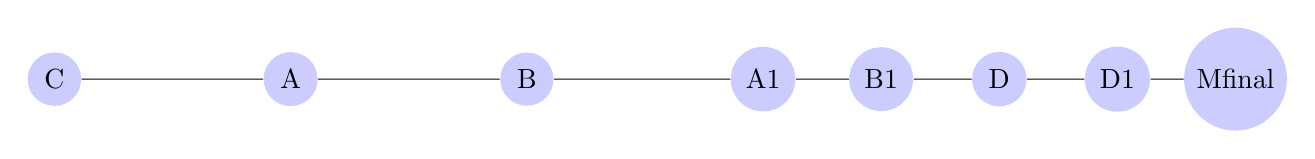
\begin{tikzpicture}
  [scale=1.5,auto=left,every node/.style={circle,fill=blue!20}]
  
  \node (n1) at (0,2)  {C};
  \node (n2) at (2,2)  {A};
  \node (n3) at (4,2)  {B};
  \node (n4) at (6,2)  {A1};
  \node (n5) at (7,2)  {B1};
  \node (n6) at (8,2)  {D};
  \node (n7) at (9,2)  {D1};
  \node (n8) at (10,2)  {Mfinal};
  \foreach \from/\to in {n1/n2,n2/n3,n3/n4,n4/n5,n5/n6,n6/n7,n7/n8}
    \draw (\from) -- (\to);
   \label{The figure for plan 1}
   \title{The figure for plan 1}
\end{tikzpicture}

\newpage
The strength for this plan is keeping each person's newest edition updated in time. However, the workflow permits only one person work in one period. When he is done, the other person can go on to update the file without overwrite it. If two person work in the same time, it requires many merges during the pulling process. As the previous graph shows, if each person push one original file and update the file for once, there will be in total 7 merges. We'll lose the efficiency of the project.\\
\\Proposal plan 2: Since A ,B ,C and D have relatively independent part of the project, each one can work on his/her own branch first, and merge to the master's branch when it is done. Considering different person may work asynchronously. Each time there's a conflict in merging, we can simply keep what it is for our own part and wait for the other one to update their part. Since C is responsible for timeline, it can be done independently in one file. If eventually C finished first, then A, B, D can follow the timeline to do their part and update their work in a fixed schedule. If C haven't finish his part, then A, B, D can work in a free way as long as they pull the latest edition from the github before they start working on their part. \\
\\Strength: Each one of the team will have its independent part, so that we can reduce the number of merge conflicts. Thus it will reduce a lot of time in merging part.
\\Weakness: the merging part will be a headache when B merged his file with master branch if  A, C, D  still work on the old edition. So someone from A, C, D needs to resolve the conflicts of merge the work of B. 

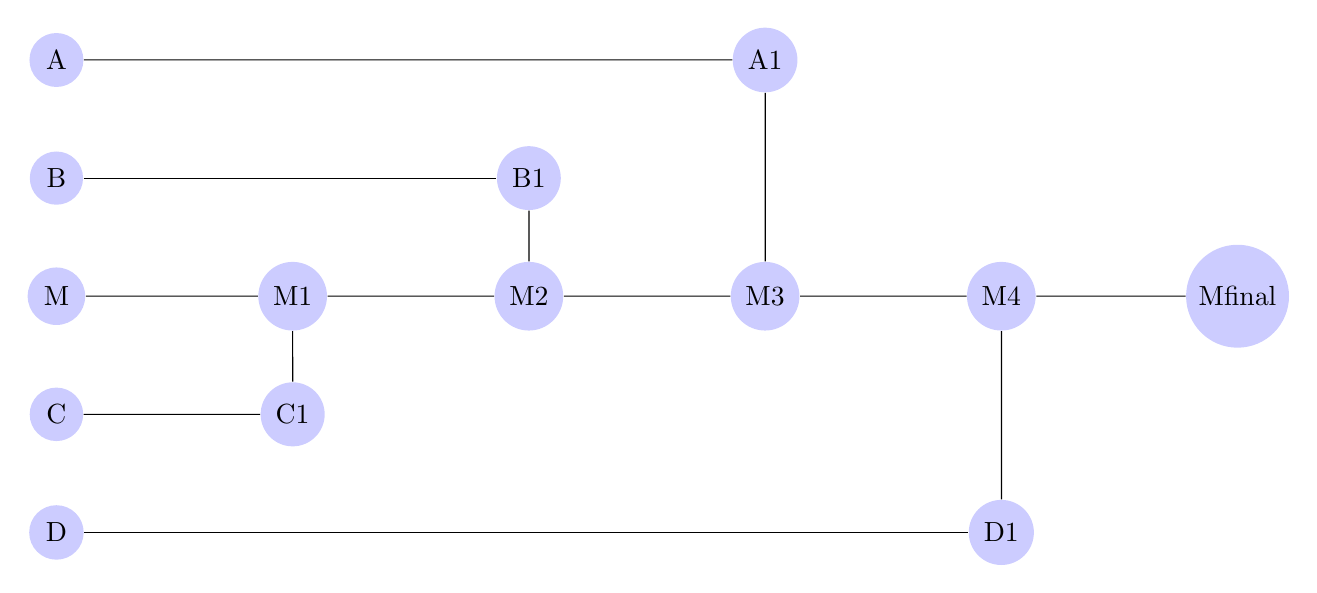
\begin{tikzpicture}
  [scale=1.5,auto=left,every node/.style={circle,fill=blue!20}]
  \node (n1) at (0,4) {A};
  \node (n2) at (0,3)  {B};
  \node (n3) at (0,2)  {M};
  \node (n4) at (0,1) {C};
  \node (n5) at (0,0)  {D};
  \node (n6) at (2,2)  {M1};
  \node (n7) at (4,2)  {M2};
  \node (n8) at (6,2)  {M3};
  \node (n9) at (8,2)  {M4};
  \node (n10) at (10,2)  {Mfinal};
  \node (n11) at (6,4) {A1};
  \node (n12) at (4,3) {B1};
  \node (n13) at (2,1) {C1};
  \node (n14) at (8,0) {D1};


  \foreach \from/\to in {n3/n6,n6/n7,n7/n8,n8/n9,n9/n10,n1/n11,n2/n12,n4/n13,n5/n14,n11/n8,n12/n7,n13/n6,n14/n9}
    \draw (\from) -- (\to);

\end{tikzpicture}

Final Recommendation: plan 2 will be better. Compared with plan 1, plan 2 has same number of editions and less merging conflicts,  which will save time effectively. On the other hand, each member of the team can keep track of the others work (individual branch) while have a clean idea of the main project (master branch).



\vskip0.25in
\noindent\textbf{Problem 4 (aka.\ Fair Play, 40 pts):}
Answer the following question:
\begin{verse}
Is the tennis game fair?
\end{verse}
Note that unlike Problem 3, this question is vaguely stated.
This is intensional, whence to begin, you will first need to clarify
what exactly your question is.
You may use the class discussion on this particular 
problem, but you \emph{may not} directly refer to our 
discussion.  Instead, formulate the model carefully but concisely in 
your own words.   

\vskip0.25in

\noindent\textbf{Original Problem:}  
\\ Is the game fair? A general standard for this is if the roles of the competitors are reversed, their probability of
winning does not change. Our original problem can be broken down to several parts: whether the player who is first to serve will be in advantage?  What will be the chances for the first game server to win the match given the probability of winning rate for each ball? And to what extent will the advantage be?\\

\noindent\textbf{Outline for the model:}  Based on the winning rate of each game, we can infer the probability that the first server to win the match. According to tennis rule, one player delivers the ball to start the game, called server; and one player receives the ball, called receiver. We simplified the rule so that any person who wins two straight points will win the game. The person who wins 6 games is the winner in a match. The possible conditions for a game are presented as following:

\begin{figure}[h]
    \begin{center}
        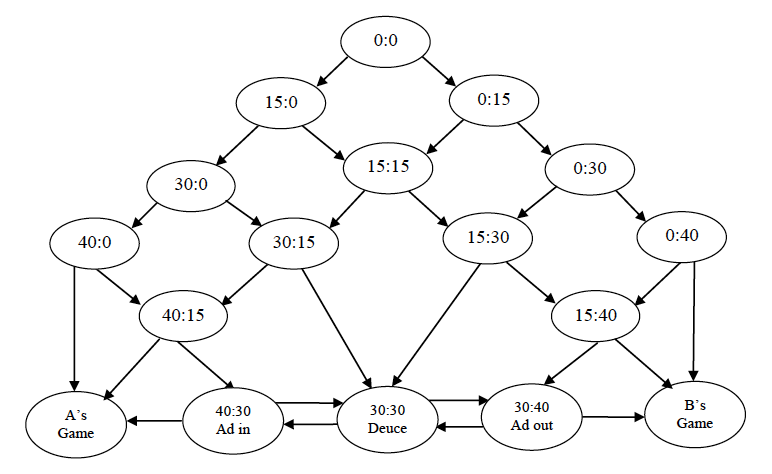
\includegraphics[scale=0.6]{graph2.png}
    \end{center}
    \caption{The graph for possible score results}
    \label{fig:branch}
\end{figure}


Condition: For both players, the chances for the server to win is $P$, and the probability for the receiver is $1-P$. \\

\noindent\textbf{Formulate the Problem:}  Whether or not the game is fair depends on the server's winning rate $P$ on each ball. For each player, the chance to win a game is the same, it equals $Q=P^2/(P^2+(1-P)^2)$. The chance to lose the game is $(1-P)^2/(P^2+(1-P)^2)$.  If P$>$1/2, then the winning rate for the server in each game is bigger than 1/2. Given the rule for winning a tennis match is the one who wins the first 6 games will win. The final score can be ``6:0", ``6:1" , ``6:2", etc.  The total chance for the first server to win is 

\[
 \sum_{k=0}^{5} {k+5\choose 6}{Q^6(1-Q)^k.}
\]
\\We are going to apply the historical data to back test the estimated rate. The best way is comparing the winning rate of each player as first-server with the winning rate as first-receiver against the same player. Then we are going to test whether there's significant difference between these two rates by two sample T-test.

The value for this function is show as following 

\begin{figure}[h]
    \begin{center}
        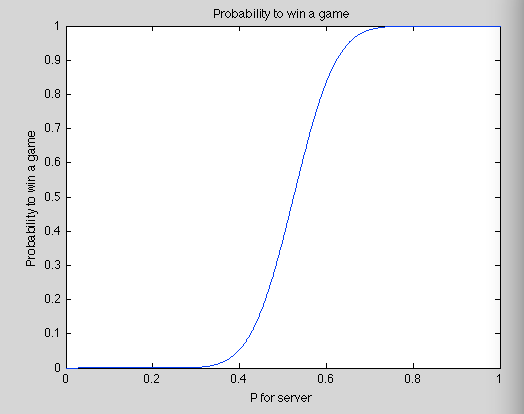
\includegraphics[scale=0.6]{graph3.png}
    \end{center}
    \caption{The graph for possible winning rate}
    \label{fig:branch}
\end{figure}

Code is as following:
\begin{figure}[h]
    \begin{center}
        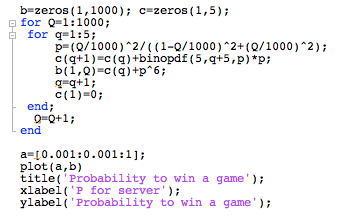
\includegraphics[scale=0.6]{code.png}
    \end{center}
    \caption{Matlab code}
    \label{fig:branch}
\end{figure}

\noindent\textbf{Is it useful?} \cite{IMM1978} 
From the model, we can infer that the fairness of tennis depends on the capability of each player. The stronger the server is, the more advantage he will possess. Especially, when $P=1/2$, the game is absolutely fair. Both receiver and server will have equal chance to win each game, thus the same probability to win the match. On the other hand, if the receiver is strong enough that the chance for him to win each point exceeds 1/2, then the game will be favorable to him. However, there are several assumptions that needs to be verified to make sure the conclusion is correct. One assumption is that winning rate in each game is constant. As we know, the result of pervious game may effect the psychological state of the players and make a difference on the next game. So the first server may have more advantage if he wins his serving game. With the historical test result, we can make the final conclusion.

\bibliographystyle{plain}
\bibliography{biblioHW}


\end{document}
